\documentclass[tikz, border=5mm]{standalone}

\usetikzlibrary{arrows,shadows,positioning}

\begin{document}

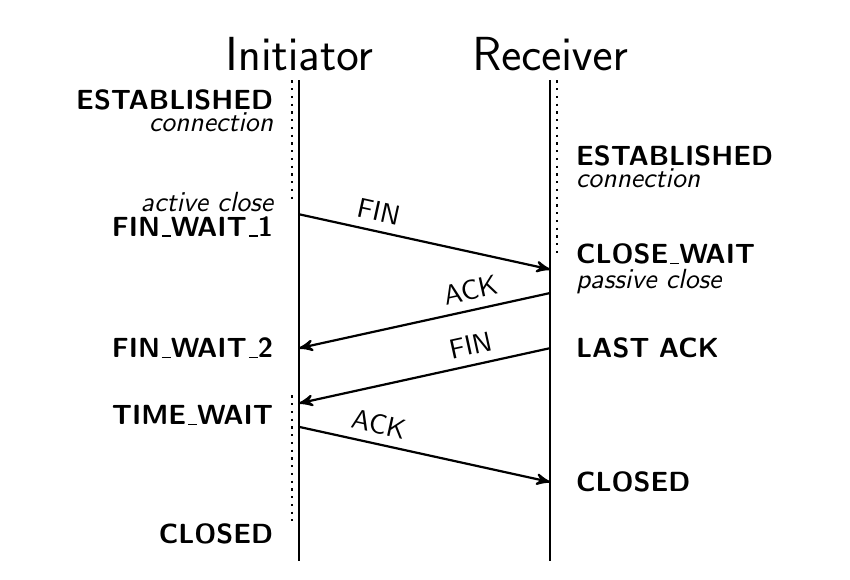
\begin{tikzpicture}[font=\sffamily,>=stealth',thick,
    commentl/.style={text width=3cm, align=right},
    commentr/.style={commentl, align=left},]
    \node[] (init) {\LARGE Initiator};
    \node[right=1cm of init] (recv) {\LARGE Receiver};


    \draw[->] ([yshift=-1.7cm]init.south) coordinate (fin1o) -- ([yshift=-.7cm]fin1o-|recv) coordinate (fin1e) node[pos=.3, above, sloped] {FIN};

    \draw[->] ([yshift=-.3cm]fin1e) coordinate (ack1o) -- ([yshift=-.7cm]ack1o-|init) coordinate (ack1e) node[pos=.3, above, sloped] {ACK};

    \draw[->] (ack1e-|recv) coordinate (fin2o) -- ([yshift=-.7cm]fin2o-|init) coordinate (fin2e) node[pos=.3, above, sloped] {FIN};

    \draw[->] ([yshift=-.3cm]fin2e) coordinate (ack2o) -- ([yshift=-.7cm]ack2o-|recv) coordinate (ack2e) node[pos=.3, above, sloped] {ACK};

    \draw[thick, shorten >=-1cm] (init) -- (init|-ack2e);
    \draw[thick, shorten >=-1cm] (recv) -- (recv|-ack2e);

    \draw[dotted] (recv.285)--([yshift=2mm]recv.285|-fin1e) coordinate[pos=.5] (aux1);

    \draw[dotted] (init.255)--([yshift=2mm]init.255|-fin1o);

    \draw[dotted] ([yshift=1mm]init.255|-fin2e) --([yshift=-5mm]init.255|-ack2e) coordinate (aux2);

    \node[commentr, right =2mm of ack2e] {\textbf{CLOSED}};
    \node[commentr, right =2mm of fin2o] {\textbf{LAST ACK}};
    \node[below left = 0mm and 2mm of init.south, commentl]{\textbf{ESTABLISHED}\\[-1.5mm]{\itshape connection}};
    \node[left = 2mm of fin1o.west, commentl]{{\itshape active close}\\[-1mm]\textbf{FIN\_WAIT\_1}};
    \node[left = 2mm of ack1e.west, commentl]{\textbf{FIN\_WAIT\_2}};
    \node[below left = -1mm and 2mm of fin2e.west, commentl]{\textbf{TIME\_WAIT}};
    \node[below left = -1mm and 2mm of aux2-|init, commentl]{\textbf{CLOSED}};

    \node[right = 2mm of recv|-aux1, commentr]{\textbf{ESTABLISHED}\\[-1.5mm]{\itshape connection}};
    \node[right = 2mm of fin1e.west, commentr]{\textbf{CLOSE\_WAIT}\\[-1mm]{\itshape passive close}};
\end{tikzpicture}

\end{document}